\chapter{User Documentation} % User guide
\label{ch:user}

In the following chapter, one could find everything he needs in order to start using Visualizing Tool. Firstly, the theory required to fully grasp all of the concepts is elaborated. Then, directions on the tool installation are provided. In conclusion, all of the parts regarding the usage of the application are explained in details.  

\section{Graphs}
Reciting the aforementioned definition - ``\emph{Graphs} are one of the unifying themes of computer science—an abstract representation that describes the organization of transportation systems, human interactions, and telecommunication networks. That so many different structures can be modeled using a single formalism is a source of great power to the educated programmer. More precisely, a graph G=(V,E) consists of a set of vertices V together with a set E of vertex pairs or edges.``~\cite{skiena-algorithm-design}. There are also two types of graphs that are worth mentioning.

\subsection{Undirected graphs}
Undirected graphs consist of the edges which are all bidirectional. Implying that if you can get from node A to node B, you will definitely be able to get from node B to node A, using the same edge. 

\begin{figure}[H]
	\centering
	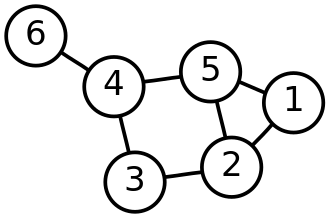
\includegraphics[width=120mm]{images/Undirected_graph_image.png}
	\caption{Undirected Graph}
\end{figure}

\subsection{Directed graphs}

In case of directed graphs, the edges have certain direction that is represented by the pointing arrow. The arrow starting at the node A, pointing at the node B, implies that you might get from A to B using the edge, but in case of directed graphs, it does not imply, that you can get from B to A.

\begin{figure}[H]
	\centering
	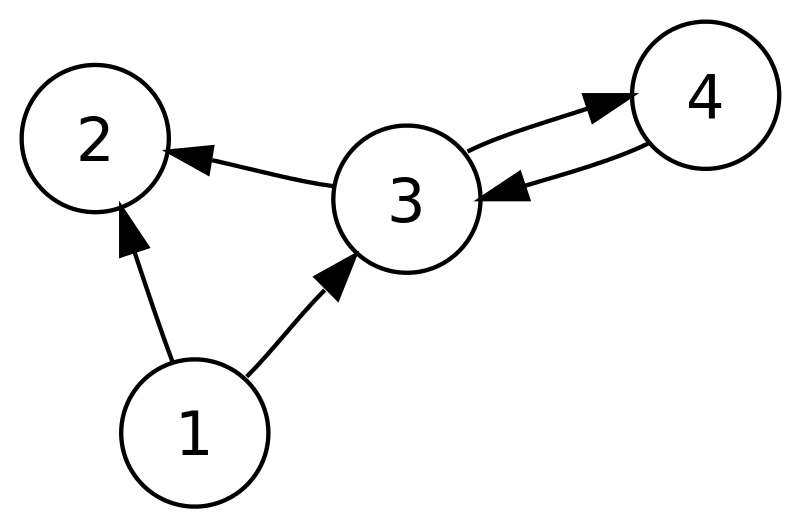
\includegraphics[width=120mm]{images/Directed_graph_image.png}
	\caption{Directed Graph}
\end{figure}

\section{Algorithms}

There are four algorithms which you are able to execute on the graphs in the tool. Such are: Breadth-first search, Depth-first search, Dijkstra and The Bellman-Ford algorithms.

\subsection{Breadth-first search}

Breadth-first search or simply BFS, is an elementary algorithm that could be used for the s-t connectivity problems. This algorithm is perfectly explained in the Cormen's book - Introduction to Algorithms.

``Breadth-first search is one of the simplest algorithms for searching a graph and the archetype for many important graph algorithms. Prim’s minimum-spanning- tree algorithm and Dijkstra’s single-source shortest-paths algorithm use ideas similar to those in breadth-first search. Given a graph G=(V,E) and a distinguished source vertex s, breadth-first search systematically explores the edges of G to "discover" every vertex that is reachable from s. It computes the distance from s to each reachable vertex, where the distance to a vertex v equals the smallest number of edges needed to go from s to v. Breadth-first search also produces a "breadth-first tree" with root s that contains all reachable vertices. For any vertex v reachable from s, the simple path in the breadth-first tree from s to v corresponds to a shortest path from s to v in G, that is, a path containing the smallest number of edges. The algorithm works on both directed and undirected graphs.``~\cite{cormen-introduction-to-algorithms}

The property of the graph which you might want to consider while executing the algorithm on the graph is whether it's weighted or not. In case, the graph is weighted it simply does not take it into account and only gives the path with minimal number of edges from A to B.

\subsection{Depth-first search}

Depth-first search or DFS, is also an elementary algorithm which also used for the pathfinding problems. Once again, Cormen explained the algorithm in well formed terms in his already mentioned book, Introduction to Algorithms.

``As its name implies, depth-first search searches "deeper" in the graph whenever possible. Depth-first search explores edges out of the most recently discovered vertex v that still has unexplored edges leaving it. Once all of v’s edges have been explored, the search "backtracks" to explore edges leaving the vertex from which v was discovered. This process continues until all vertices that are reachable from the original source vertex have been discovered. If any undiscovered vertices remain, then depth-first search selects one of them as a new source, repeating the search.``~\cite{cormen-introduction-to-algorithms}

The same concept applies to DFS as it does to BFS, it gives an optimal solution in case of unweighted graphs. Worth mentioning that it also does not give out the "shortest" path but the first lexicographical which means that if you have paths 1->2->3 and 1->4->3 it will give out the first one as the resulting path, as 2 is less than 4.

\subsection{Dijkstra}

Dijkstra's algorithm for finding the shortest paths in the weighted graph is one of the most favored in its field of purpose. It is plain and efficient, so it is widely used in different applicable areas. Skiena clearly elaborated definition of the algorithm in his book 'The Algorithm Design Manual'.

``Dijkstra’s algorithm is the method of choice for finding shortest paths in an edge and/or vertex-weighted graph. Given a particular start vertex s, it finds the shortest path from s to every other vertex in the graph, including your desired destination t.Suppose the shortest path from s to t in graph G passes through a particular intermediate vertex x. Clearly, this path must contain the shortest path from s to x as its prefix, because if not, we could shorten our s-to-t path by using the shorter s-to-x prefix. Thus, we must compute the shortest path from s to x before we find the path from s to t.Dijkstra’s algorithm proceeds in a series of rounds, where each round establishes the shortest path from s to some new vertex. Specifically, x is the vertex that minimizes dist(s,$v_i$)+w($v_i$,x) over all unfinished 1 $\leq$ i $\leq$ n, where w(i,j) is the length of the edge from i to j, and dist(i,j) is the length of the shortest path between them.This suggests a dynamic programming-like strategy. The shortest path from s to itself is trivial unless there are negative weight edges, so dist(s,s)=0.If(s,y)is the lightest edge incident to s, then this implies that dist(s,y)=w(s,y). Once we determine the shortest path to a node x, we check all the outgoing edges of x to see whether there is a better path from s to some unknown vertex through x.``~\cite{skiena-algorithm-design}

The Dijkstra algorithm works for non-negative weighted graphs, because as soon as it meets a negative edge it is stuck in the infinite loop. For the sake of user experience, all of the negative edges, in case of using Dijkstra, are treated as 0-weighted edges. In that instance, it won't find the optimal solution but it will not stay in the loop forever either, so that is an understandable sacrifice. In case of the unweighted graphs, Dijkstra finds a solution, but is not necessarily the best in this case, as you might achieve the same result by using easier algorithm such as BFS.

\subsection{The Bellman-Ford}

The Bellman-Ford algorithm is very crucial in cases when you need to find the path in the weighted graph with negative values. Though, it is more complex and resource consuming, the broader set of graphs could be resolved with the algorithm. 

By Cormen, ``it solves the single-source shortest-paths problem in the general case in which edge weights may be negative. Given a weighted, directed graph G=(V,E) with source vertex sand weight function $w : E \rightarrow \mathbb{R}$, the Bellman-Ford algorithm returns a boolean value indicating whether there is a negative-weight cycle that is reachable from the source. If there is such a cycle, the algorithm indicates that no solution exists. If there is no such cycle, the algorithm produces the shortest paths and their weights. The procedure BELLMAN-FORD relaxes edges, progressively decreasing an estimate v.d on the weight of a shortest path from the source s to each vertex $v \in V$ until it achieves the actual shortest-path weight $\delta(s,v)$. The algorithm returns TRUE if and only if the graph contains no negative-weight cycles that are reachable from the source.``~\cite{cormen-introduction-to-algorithms}

The algorithm is a great choice in cases when you have negative weights in the graph, but whenever there is a graph with no negative weights, The Bellman-Ford loses a lot due to it being executed on every edge of the graph and repeating the step until no further relaxations are possible.

\section{Installing the tool}

The tool might be used by installing some software and running couple of commands in order to start it on your local machine. It is a web application, though self-hosted app would not need any connection to the web.

\subsection{Required software}

There are two parts playing role in the application. Front end, the client-side application which plays role in everything related to view of the program and Back end, the server-side application which computes every operation that is being requested from the client.

For the back, you would need to follow the next steps:
\begin{itemize}
	\item[1] Install Python 3.12~\cite{python-download-web}
	\item[-] (Optional) Install PyCharm~\cite{pycharm-download-web}
	\item[2] Go into the directory - app
	\item[3] Run the command for the installation of the packages
	\begin{lstlisting}[language={bash}]
		pip install -rrequirements.txt
	\end{lstlisting}
	\item[4] Go back to the previous directory
	\item[5.1] After that you can run the application using the next command
	\begin{lstlisting}[language={bash}]
		python app/main.py
	\end{lstlisting}
	If you are having an error, you might want to check whether your current PYTHONPATH environmental variable is set appropriately, to the directory of the whole project. There is an example of its usage in the github ci workflow file.
	\item[5.2] In case of using PyCharm, go to the main.py file and execute the main by clicking the run button. 
\end{itemize}



For the front, you would need to follow the next steps:
\begin{itemize}
	\item[1] Install Node.js~\cite{nodejs-web} (v20.x.x LTS)
	\item[2] Go into the directory - app-view
	\item[3] Run the command for the installation of the packages
		\begin{lstlisting}[language={bash}]
			npm install
		\end{lstlisting}
	\item[4] After that you can run the application using the next command
		\begin{lstlisting}[language={bash}]
			npm start
		\end{lstlisting}
	\item[5] The window will open in your default browser, if it doesn't then open the website on the URL - http://localhost:3000/.
\end{itemize}

\section{Manual on the tool}

There are two main capabilities of the tool that this manual will mostly be about: graph and algorithm control. So, let's cover those parts in details for the sake of understanding on how to use the tool.

\subsection{Main pages}

The tool meets you with a nice welcome page and a navigation bar. The learner has such options as undirected and directed graphs.

\begin{figure}[H]
	\centering
	
\includegraphics[width=\textwidth]{images/welcome_page.png}
	\caption{Welcome Page}
\end{figure}

On the figure 2.4 one might see the empty graph page. The initial states of the undirected and directed pages are indistinguishable as long as the user won't create a graph. Further on the manual, the undirected graph page will be used to demonstrate the functionality of the tool. Division into five main components could be derived from the page. These are communication panel, graph canvas, algorithm description panel, graph control panel and algorithm control panel. The communication, canvas and description panels are separated by gray borders and the remaining panels are located below them.

\begin{figure}[H]
	\centering
	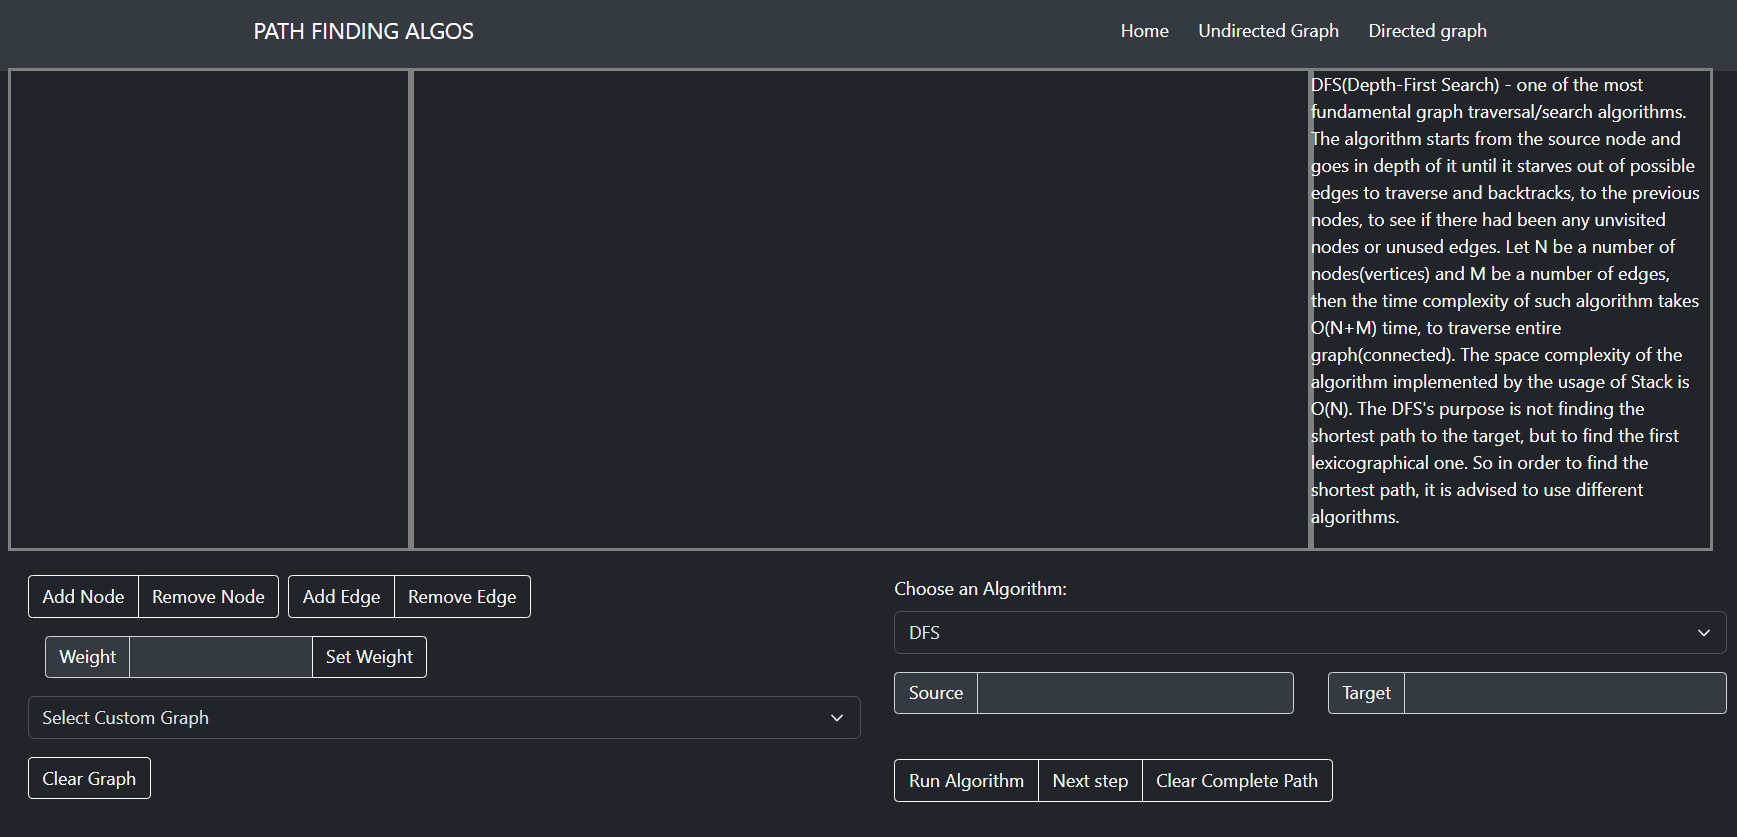
\includegraphics[width=\textwidth]{images/empty_graph_page.png}
	\caption{Empty Graph Page}
\end{figure}

\subsection{Adding node}

The node addition does not require anything but the click of a single button on the graph control panel side of the page. "Add Node" button is used to create a new node on the page. New node is going to pop out in the random location on the canvas. And a message in the communication panel will appear saying "Added node!" which indicates that the node has been added to the graph successfully.

\begin{figure}[H]
	\centering
	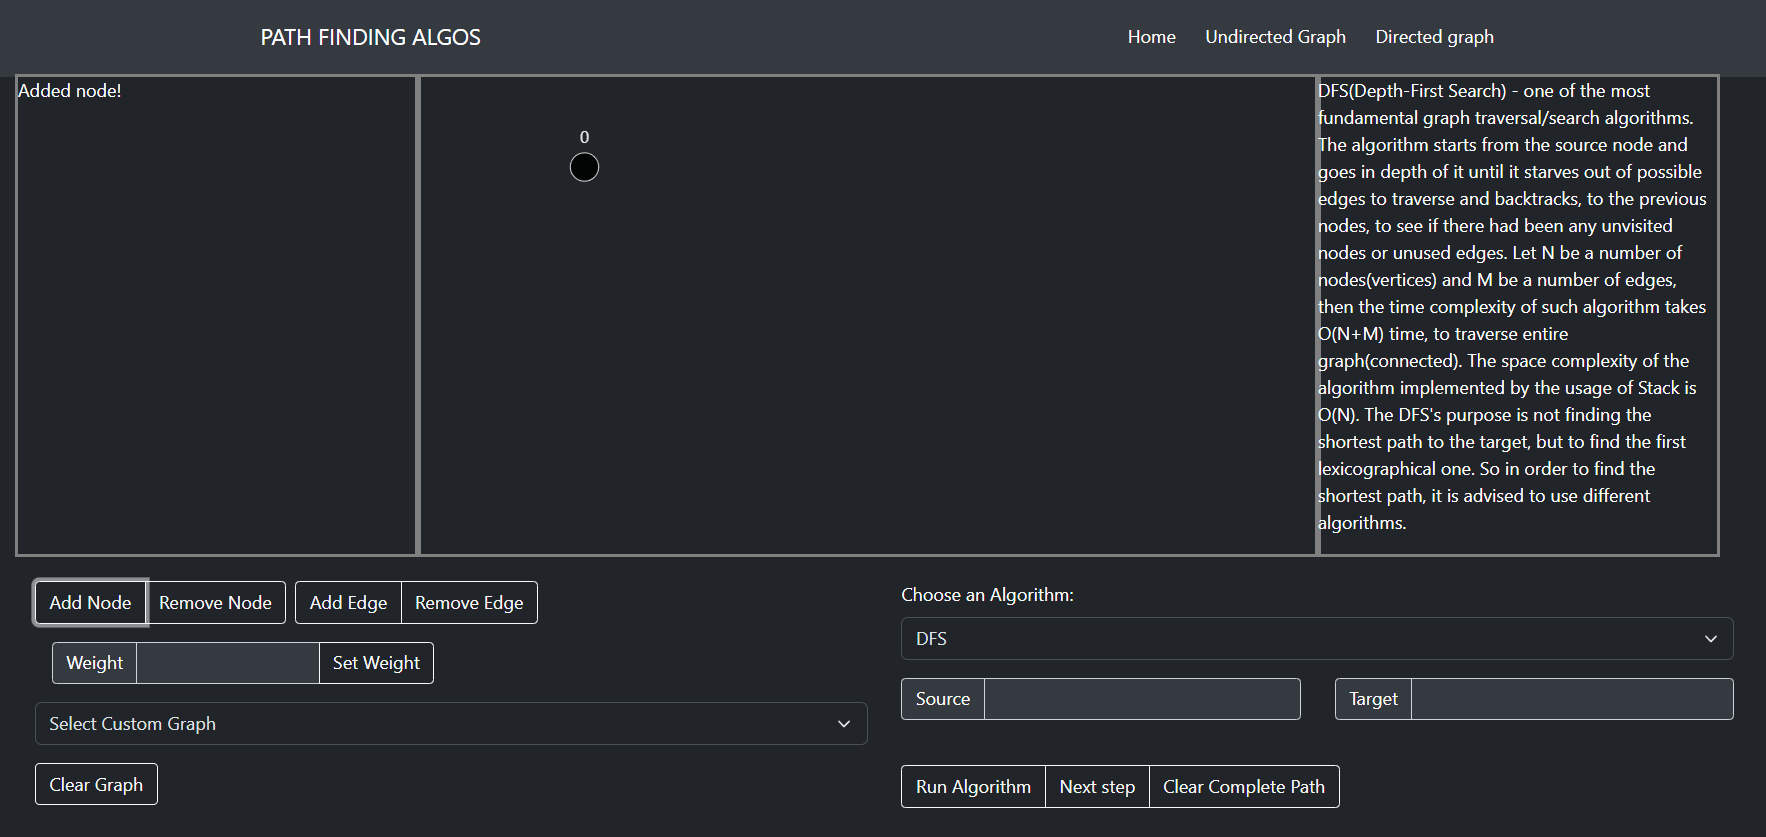
\includegraphics[width=\textwidth]{images/add_node_to_graph.png}
	\caption{Adding node to graph}
\end{figure}

\subsection{Removing node}

In order to remove the node, you must have at least one node in the graph. "Remove node" button in the graph control panel let's us to choose any node in the graph that we would like to delete.

\begin{figure}[H]
	\centering
	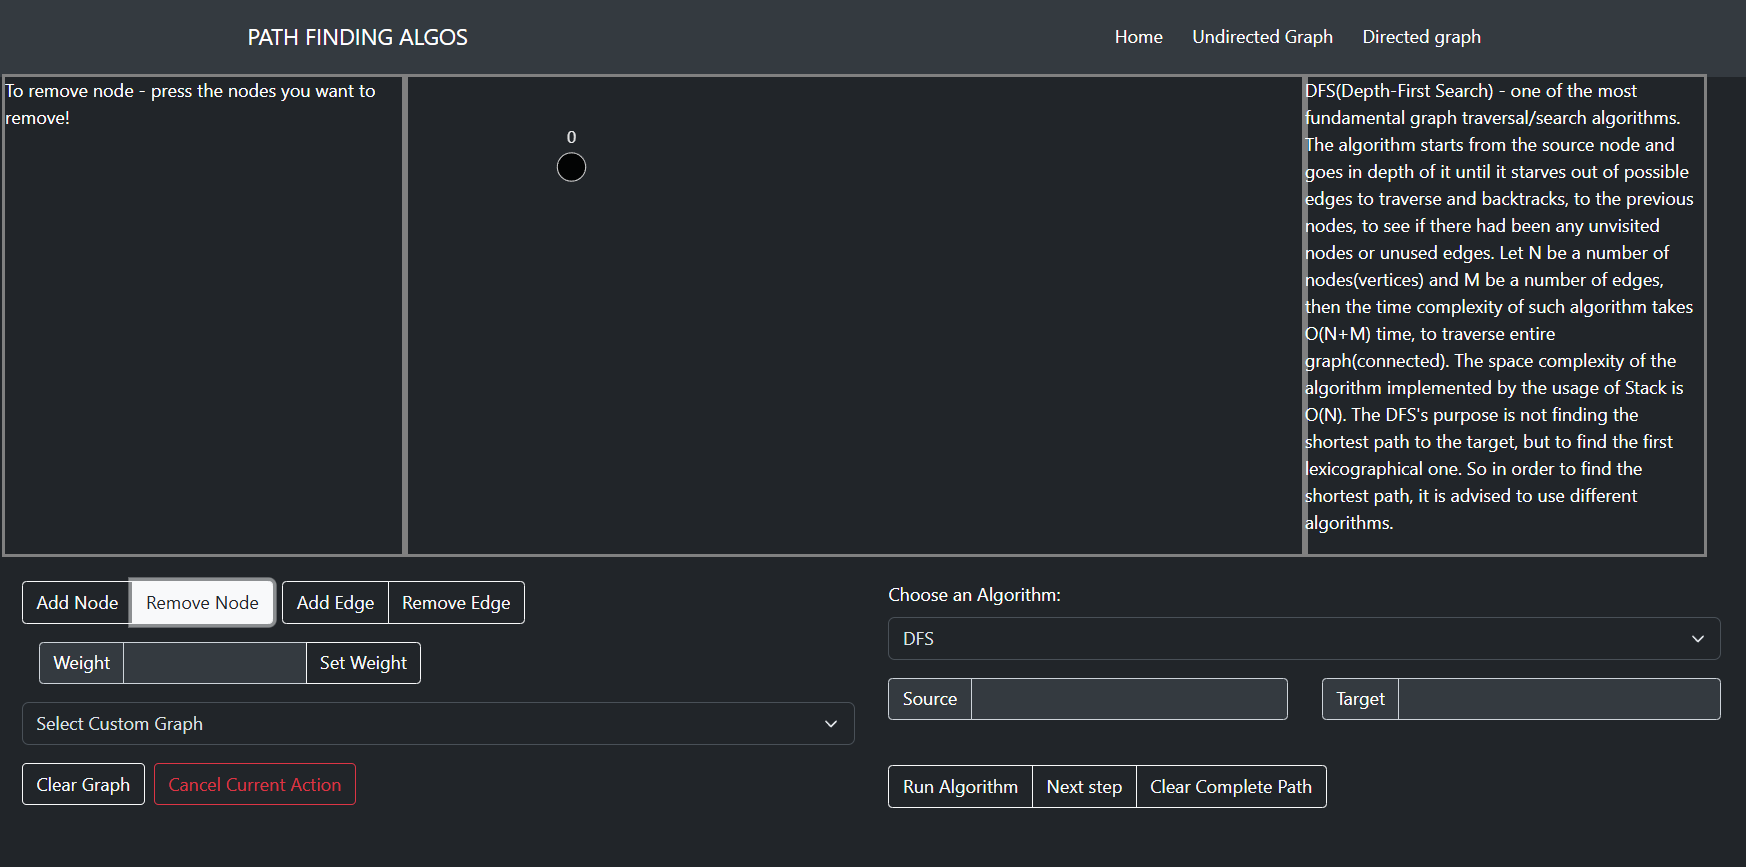
\includegraphics[width=\textwidth]{images/removing_node.png}
	\caption{Removing node from graph}
\end{figure}

After pressing such button and clicking on any node of the graph, the chosen node will be removed and the relevant message will appear. All of the nodes, which had the bigger index will be decreased by one and in case there is at least one node with the larger index in the graph, it will take the place of the removed one after deletion. Such behavior is caused by the limitation of library used for drawing of graph on the screen.

\begin{figure}[H]
	\centering
	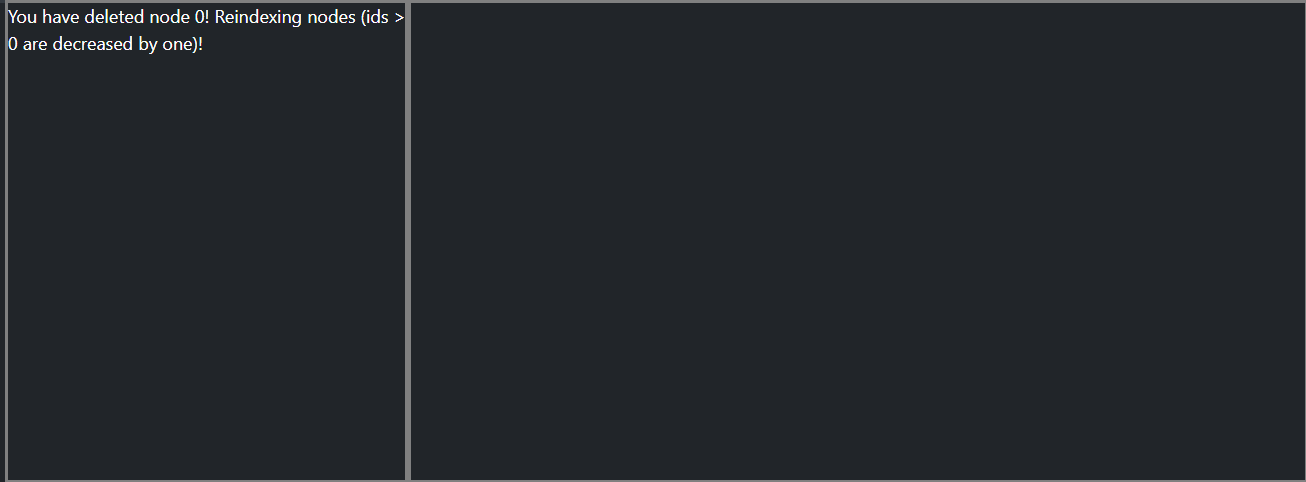
\includegraphics[width=\textwidth]{images/removed_node.png}
	\caption{Removed node from graph}
\end{figure}

\subsection{Adding edge}

The addition of the edge is achieved by the click of the button "Add Edge" and further steps of choosing the nodes between which the edge shall appear. 

\begin{figure}[H]
	\centering
	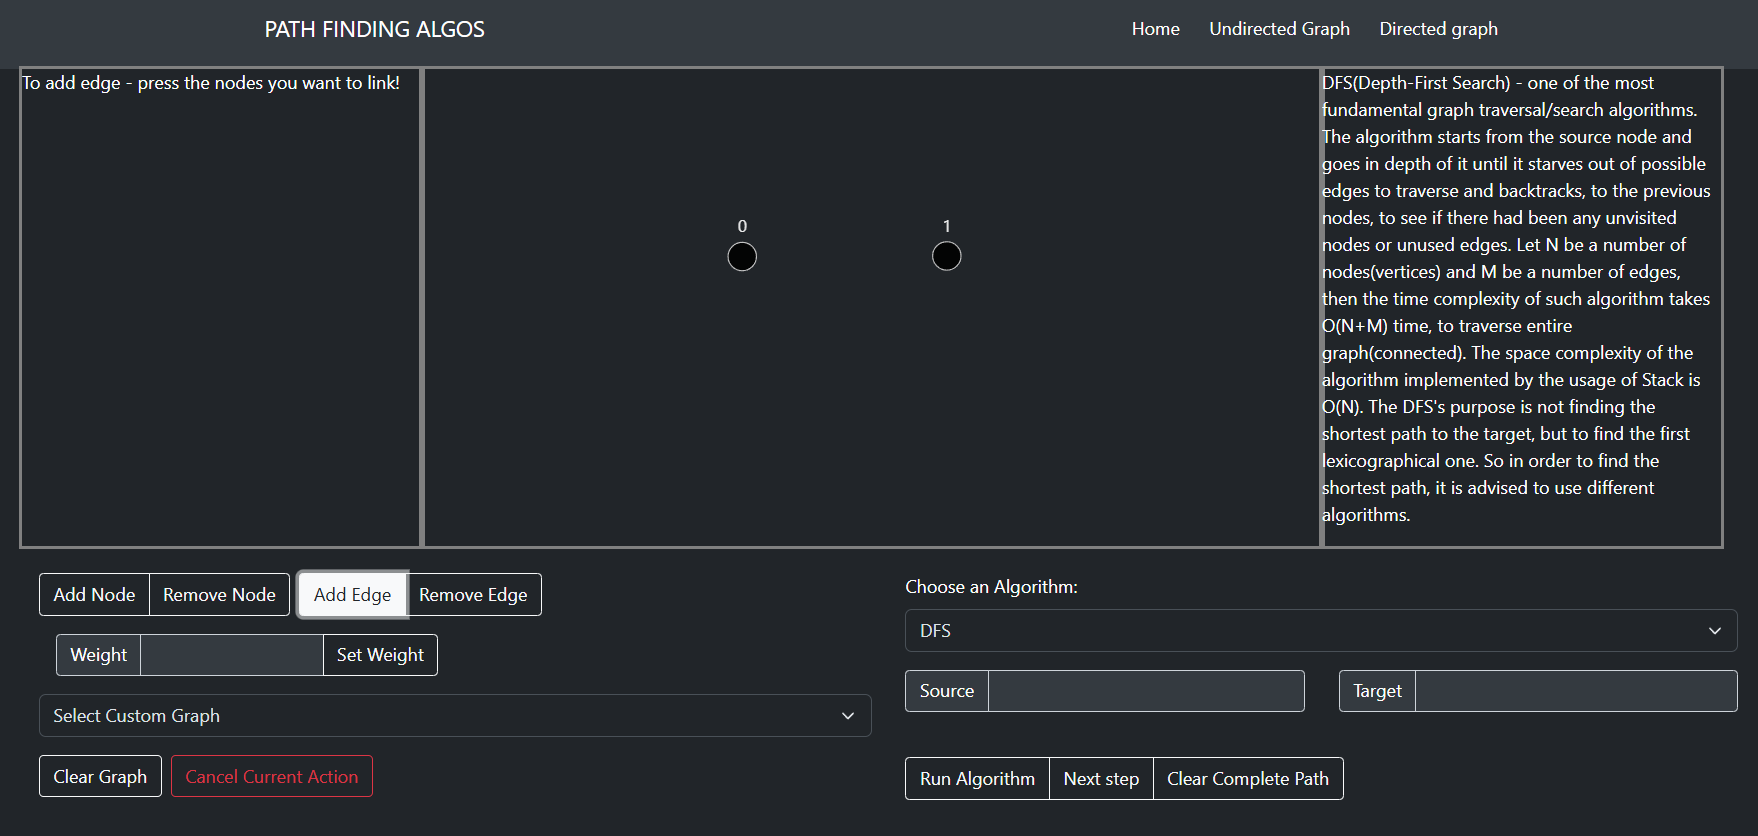
\includegraphics[width=\textwidth]{images/adding_edge.png}
	\caption{Adding edge to graph}
\end{figure}

After you have clicked on the first node you will see the message appear, indicating that you have successfully chose out-node, the node from which edge will lead into the other node(in case of directed graphs).

\begin{figure}[H]
	\centering
	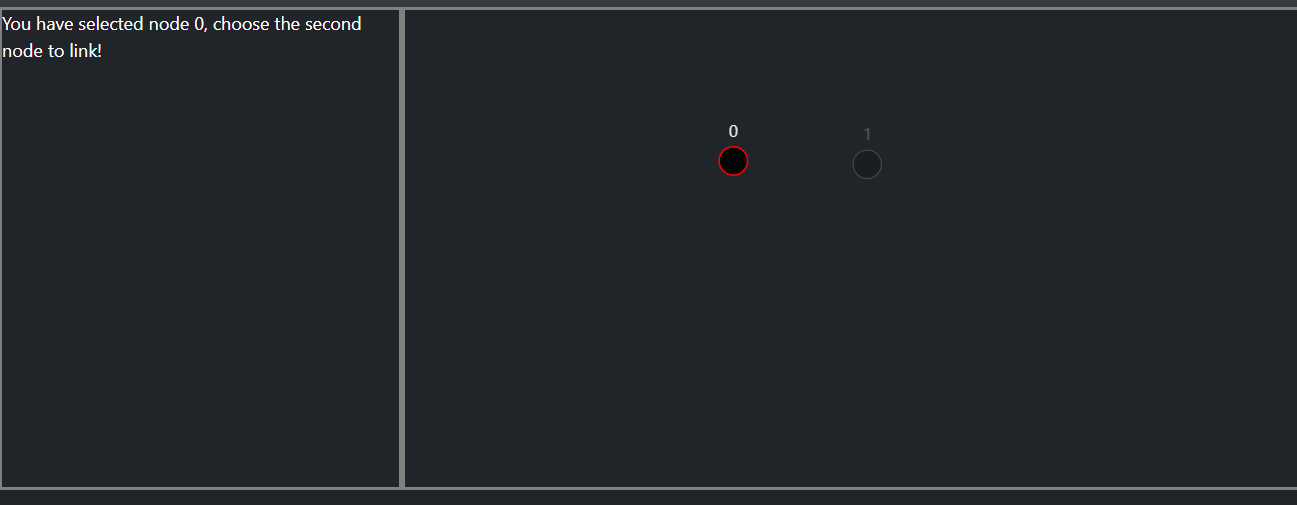
\includegraphics[width=\textwidth]{images/adding_edge_select_first_node.png}
	\caption{Selecting first node}
\end{figure}

Finally, if you have chosen a proper node to be the in-node, then the edge will be created between them. Additionally, The message will indicate the success of the operation.

\begin{figure}[H]
	\centering
	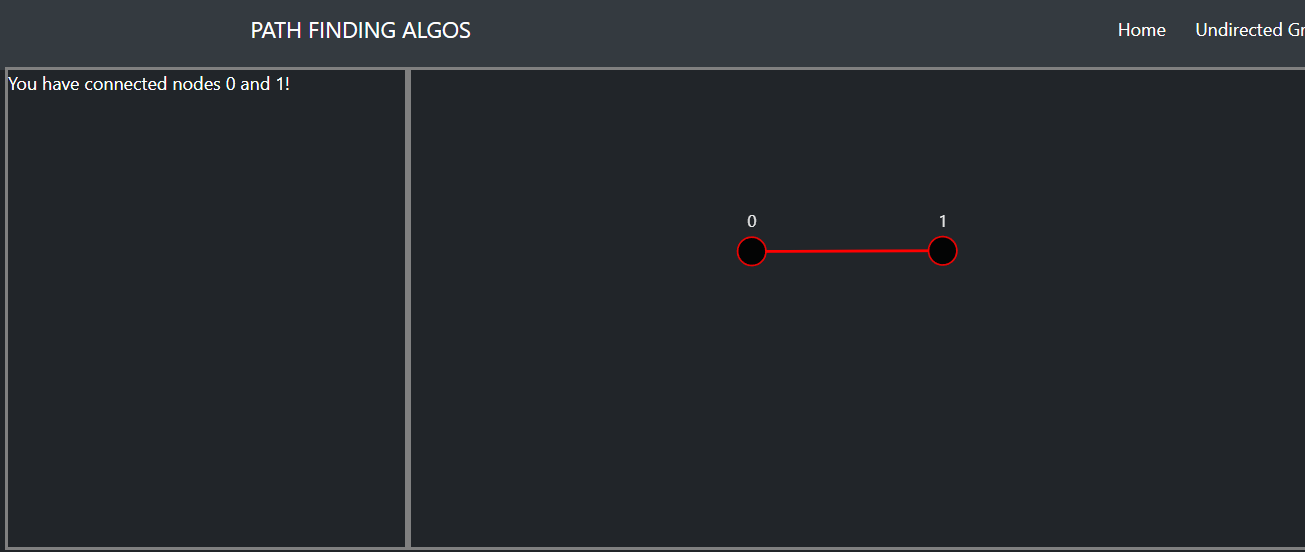
\includegraphics[width=\textwidth]{images/added_edge.png}
	\caption{Selecting second node}
\end{figure}

\subsection{Removing edge}

Removal of the edge appears to be quite similar to the operation of node removal. One must click on the "Remove edge" button to see that the communication panel is telling them to choose any edge they want to delete.

\begin{figure}[H]
	\centering
	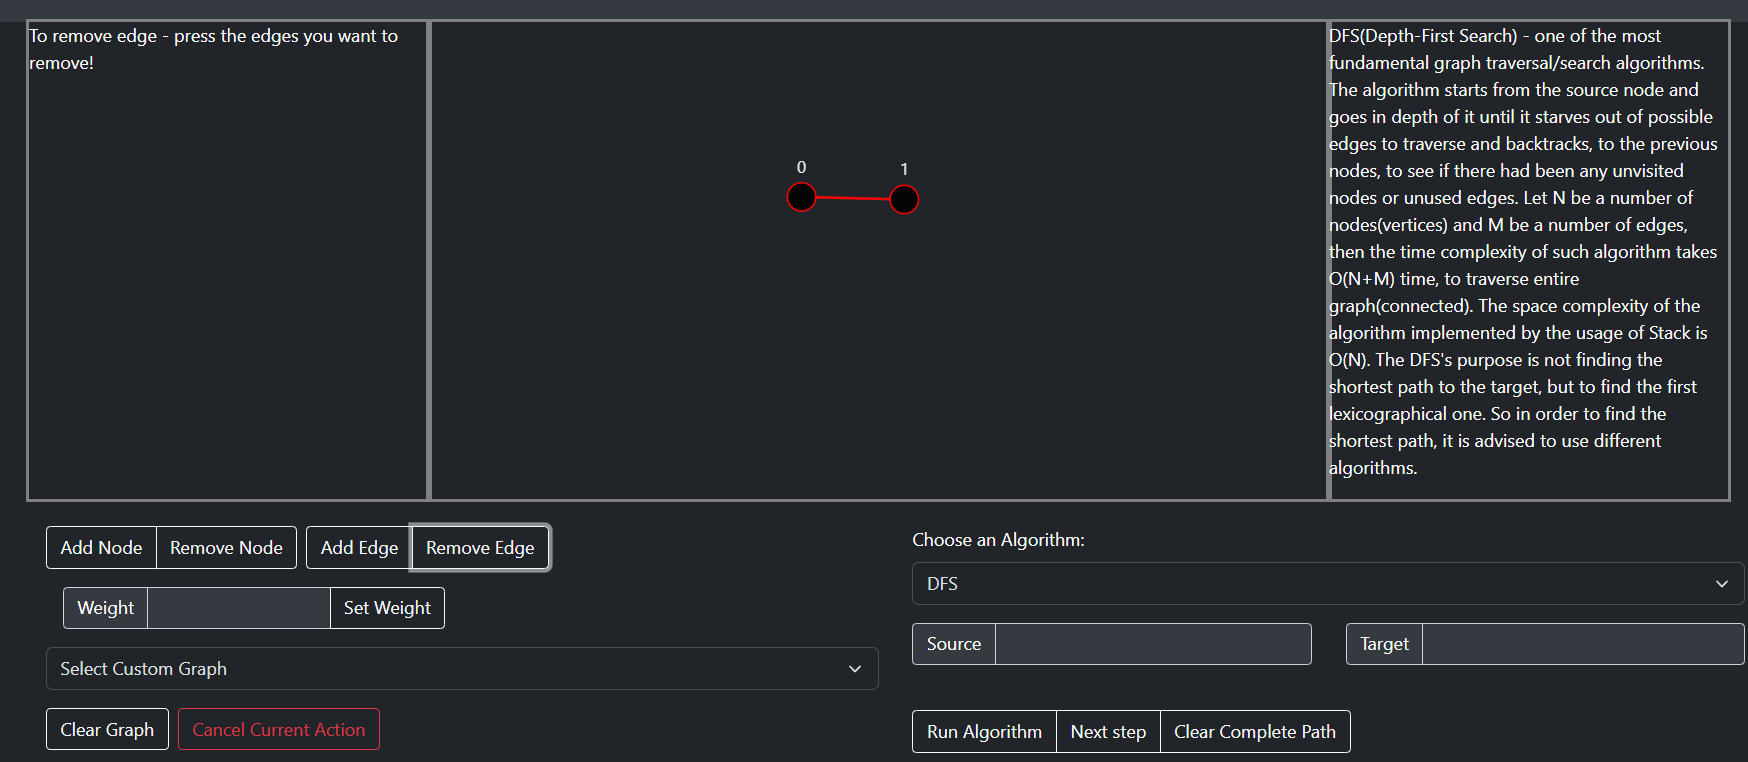
\includegraphics[width=\textwidth]{images/removing_edge.png}
	\caption{Removing edge from graph}
\end{figure}

By following the instructions of the communication panel seen on the figure 2.11, the successful removal of the chosen edge is achieved. Also, worth mentioning, that the removal of the edge may be executed by the removal of the node as well, in case the deleted node has any incoming or outgoing edges.

\begin{figure}[H]
	\centering
	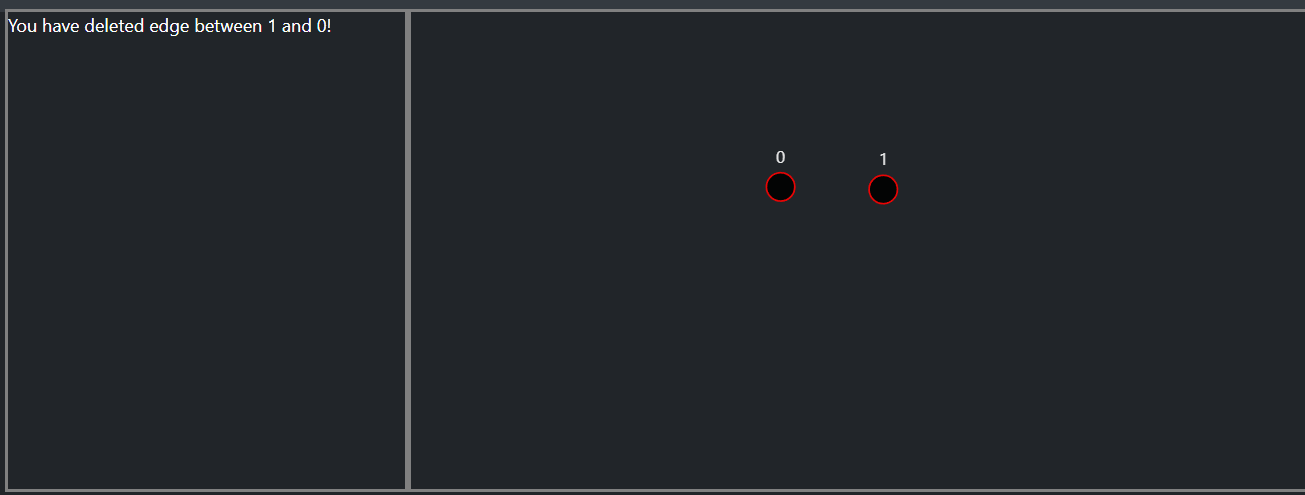
\includegraphics[width=\textwidth]{images/removed_edge.png}
	\caption{Removed edge from graph}
\end{figure}

\subsection{Setting the weight for the edge}

The weighted graphs are needed, if the learner wants to see the execution of such algorithms as 'Dijkstra' and 'The Bellman-Ford' in environment they are the best fit for. So, this option is available, which user might notice on the graph control panel. First of all, you need to specify the weight that you want your edge to have. This is achieved by clicking on the weight numerical input bar. One might input their desired weight by using the arrows which increase or decrease the number or write it down using keyboard.

\begin{figure}[H]
	\centering
	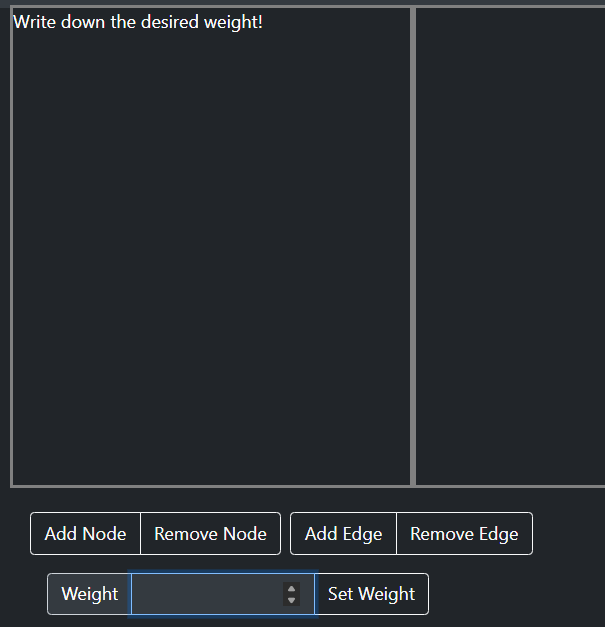
\includegraphics[width=\textwidth]{images/writing_the_weight_number.png}
	\caption{Writing down the weight number}
\end{figure}

Secondly, user needs to click on the "Set Weight" button. After that, the message will inform that you are free to choose from the edges on a graph to set the weight for it.

\begin{figure}[H]
	\centering
	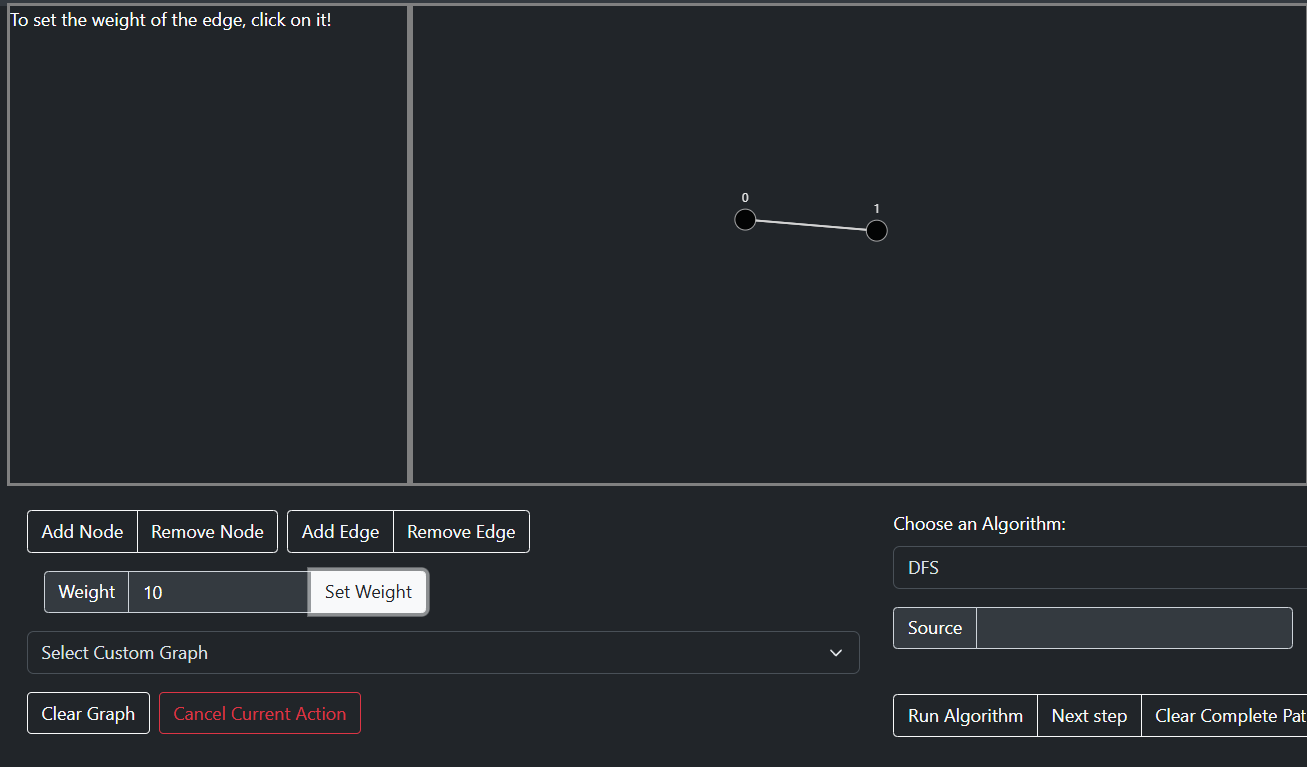
\includegraphics[width=\textwidth]{images/setting_the_weight_for_the_edge.png}
	\caption{Setting the weight for an edge}
\end{figure}

After completion of the previous instruction, the weight appears on the chosen edge. For the sake of clarity, communication panel shows the node indices between which the edge has been chosen to gain a weight.

\begin{figure}[H]
	\centering
	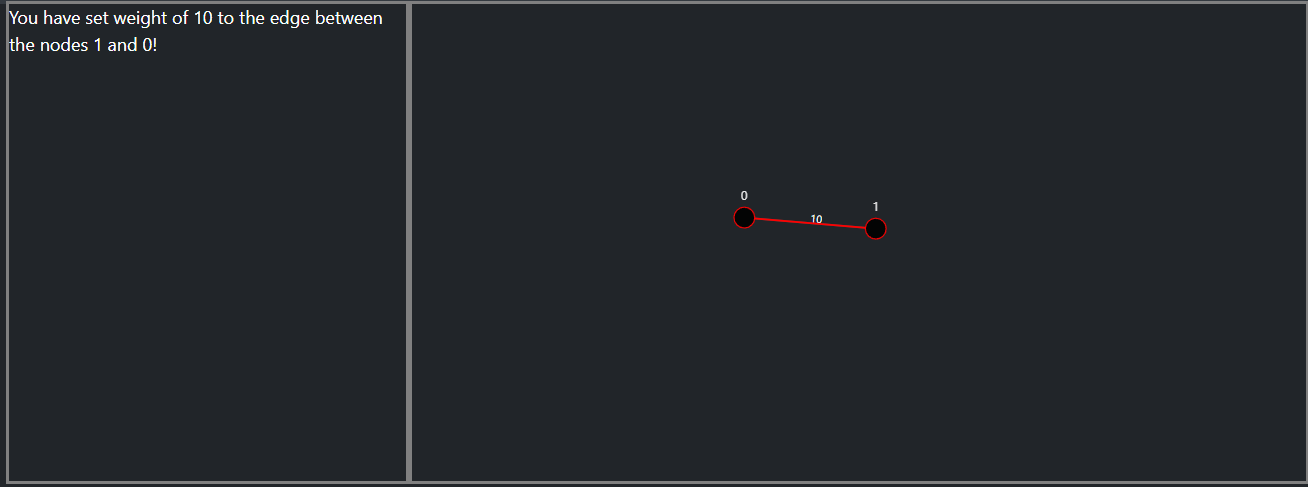
\includegraphics[width=\textwidth]{images/set_the_weight.png}
	\caption{Set the weight}
\end{figure}

\subsection{Choosing from prepared graphs}

The tool does not support importing of the custom graphs yet. However, user might chose from the ones that are already built-in. All that needs to be done is the click on "Select Custom Graph" selection box and the further choice of graph which needs to be imported for the client.

\begin{figure}[H]
	\centering
	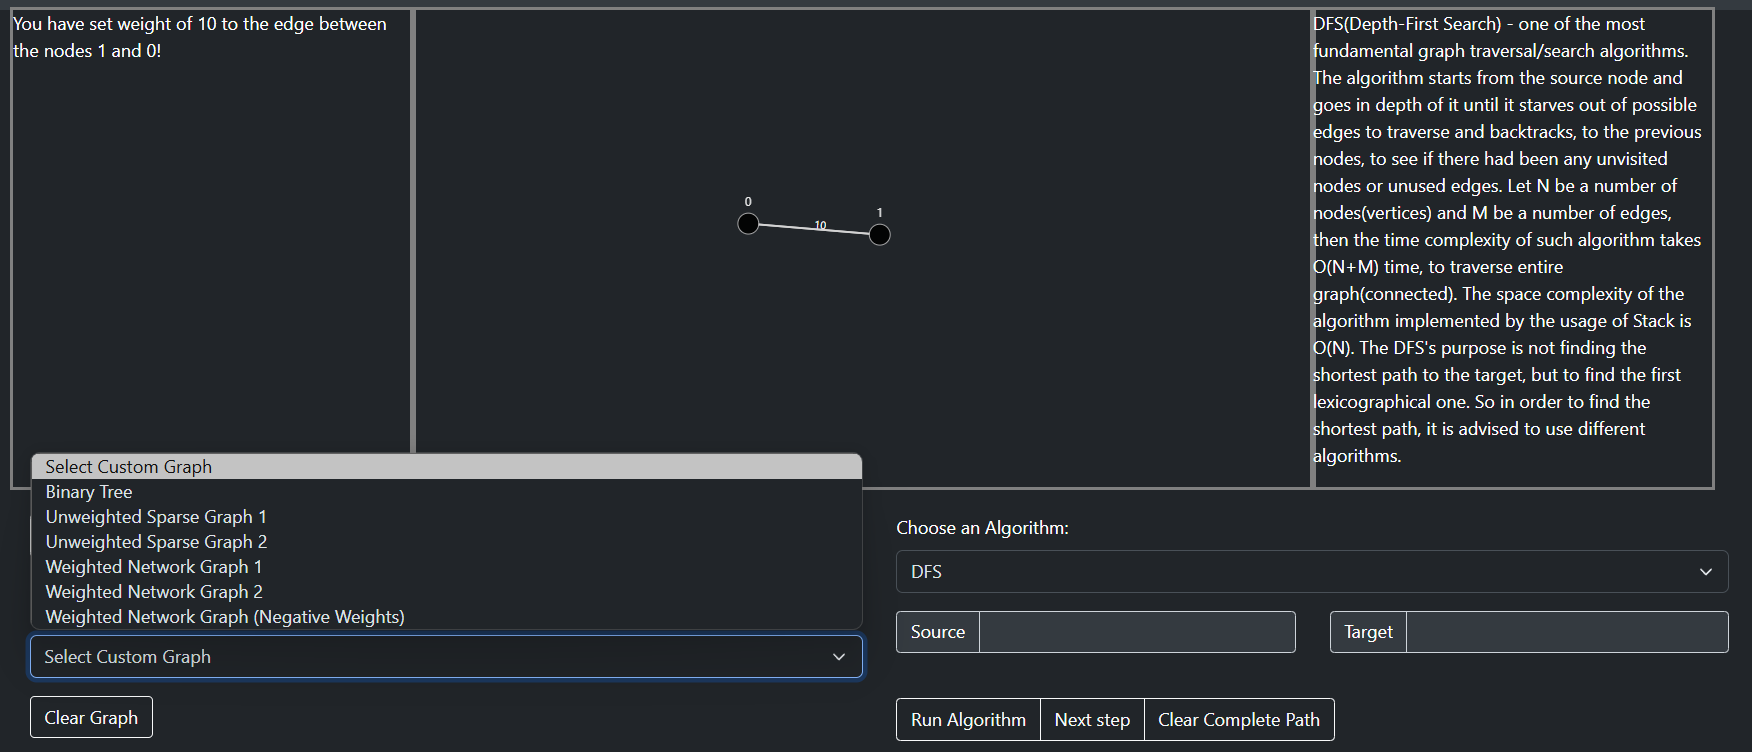
\includegraphics[width=\textwidth]{images/selecting_prepared_graph.png}
	\caption{Selecting from prepared graphs}
\end{figure}

\subsection{Canceling action}

After certain actions, such as removing nodes and edges, addition of the edge and setting of weight one has an option to revoke the chosen operation by the "Cancel Current Action" button. It appears every time one of the actions listed in the previous sentence is being executed.

\begin{figure}[H]
	\centering
	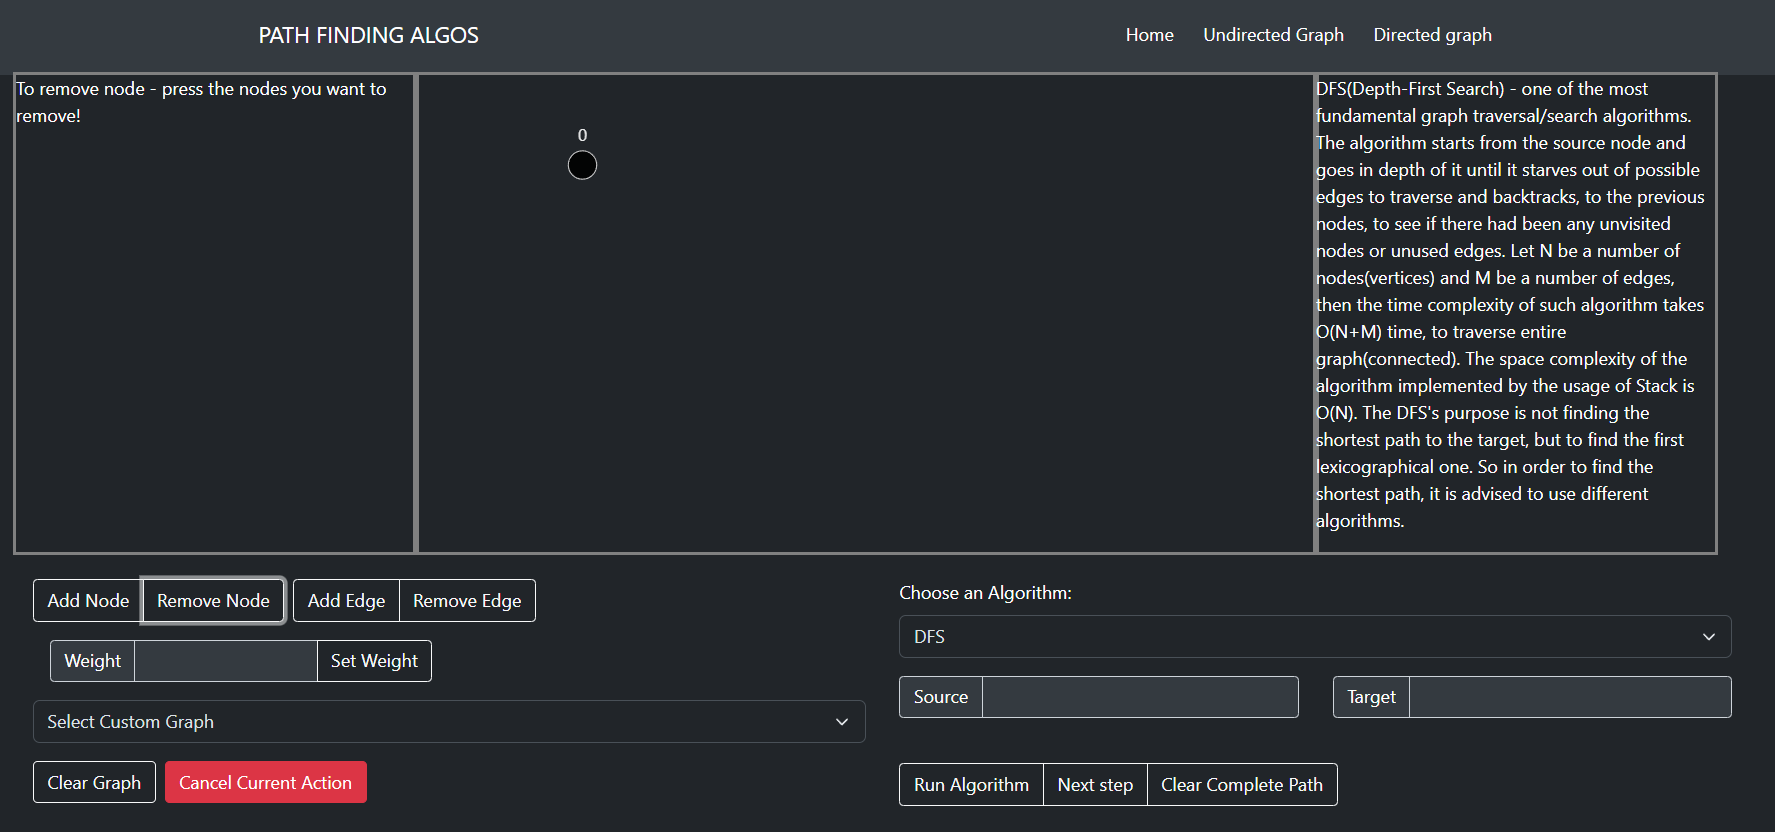
\includegraphics[width=\textwidth]{images/cancel_current_action.png}
	\caption{Cancel ongoing action}
\end{figure}

\subsection{Choosing the algorithm}

Now, switching focus to the algorithm control panel, there is a "Choose an Algorithm" selection box. By using it, learner can change the current algorithm that they would like to be executed on the graph to be chosen. There are four choices such as DFS, BFS, Djikstra and the Bellman-Ford. 

\begin{figure}[H]
	\centering
	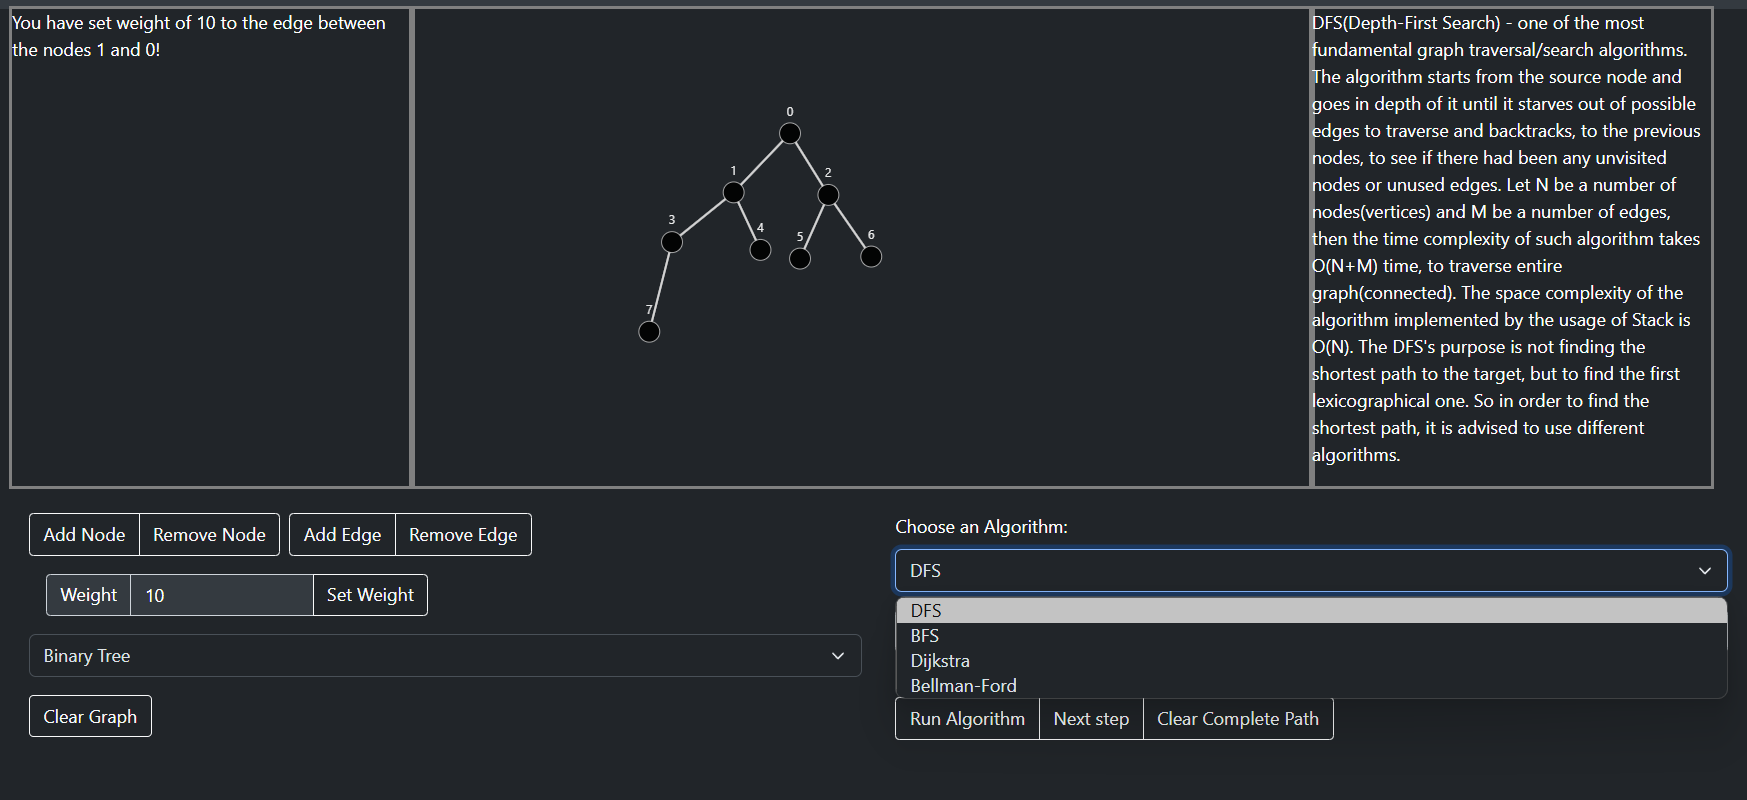
\includegraphics[width=\textwidth]{images/choosing_the_algorithm.png}
	\caption{Choose the algorithm}
\end{figure}

\subsection{Running the algorithm}

When one has the complete graph, the algorithm can be executed. Though, there are couple of preparation steps they would need to follow. Initially, choose the source and target nodes from the graph. User can choose these by clicking on the relevant source and target read-only input boxes and then clicking on the nodes they want to select as a source or target. The order is clear, if one follows instructions of the communication panel.

\begin{figure}[H]
	\centering
	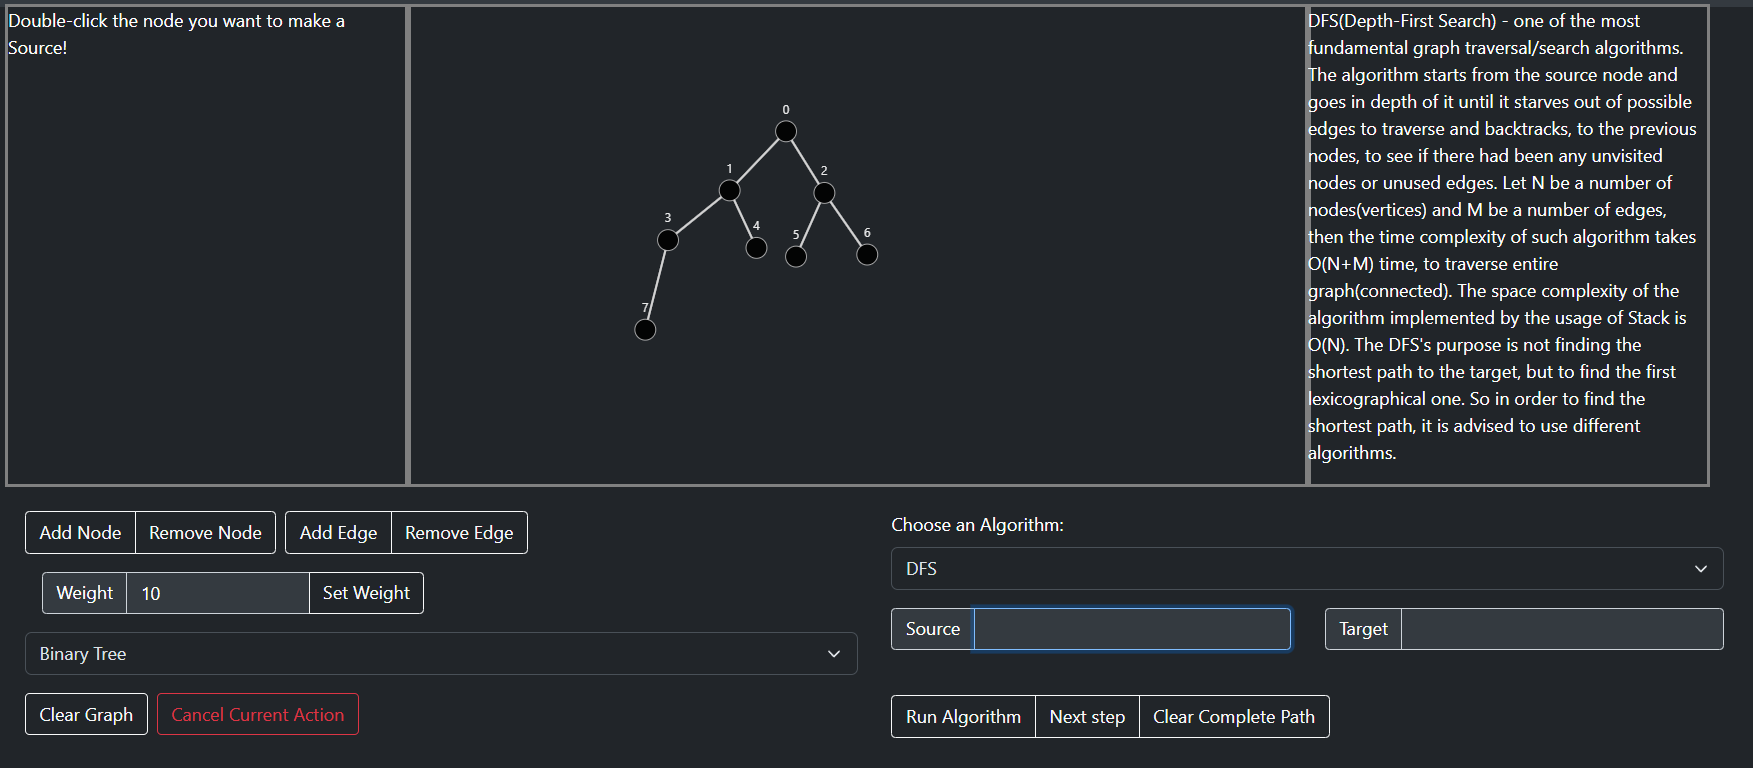
\includegraphics[width=\textwidth]{images/choosing_source_node.png}
	\caption{Choose the source node}
\end{figure}

As we have the source and target nodes, we might continue with the execution. In order to proceed, there is a "Run Algorithm" button, which one shall click.

\begin{figure}[H]
	\centering
	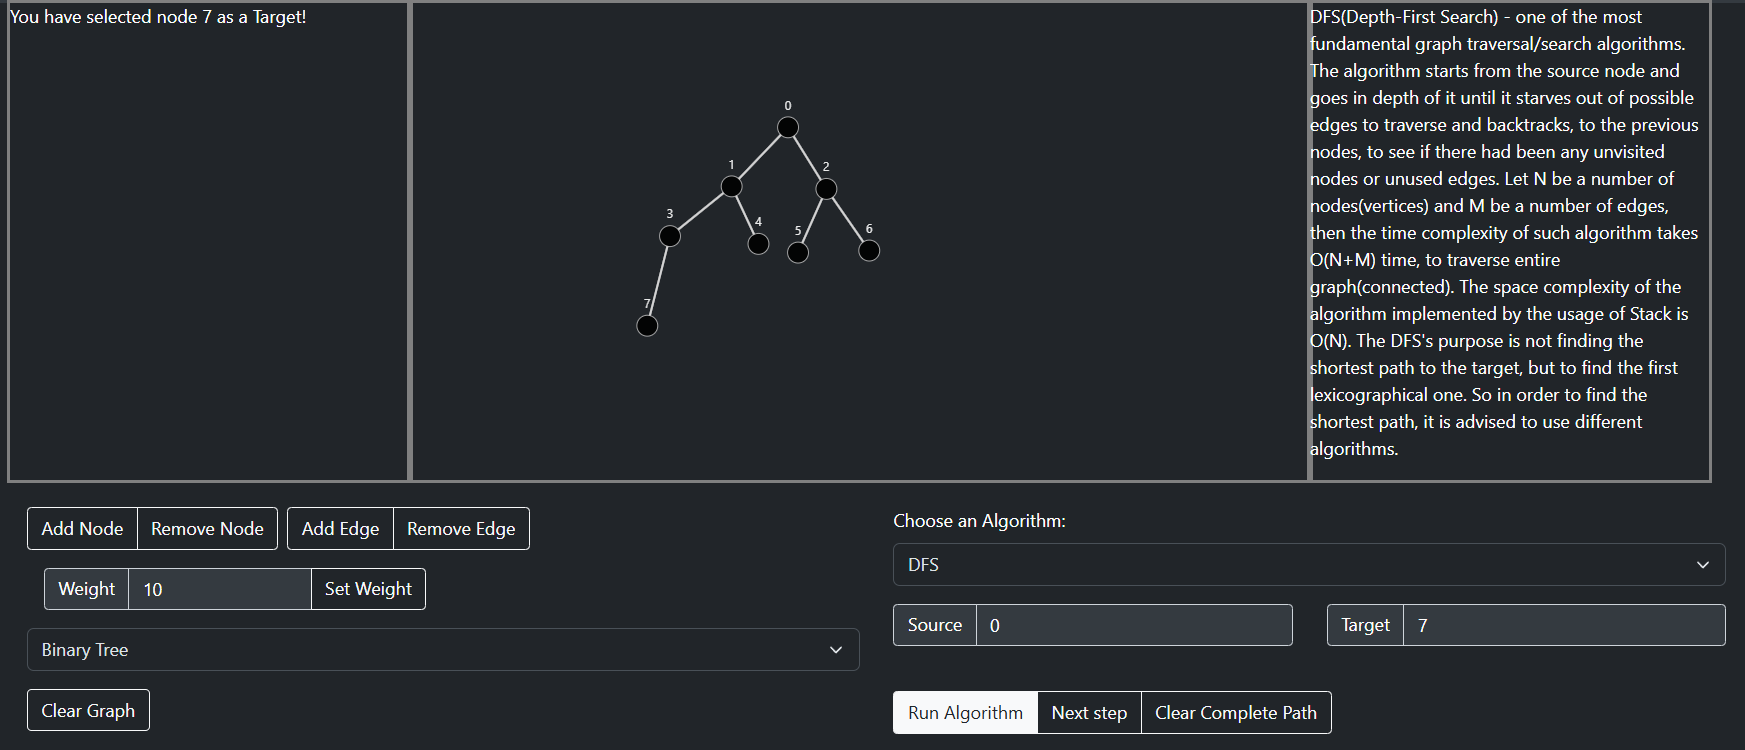
\includegraphics[width=\textwidth]{images/running_the_algo.png}
	\caption{Running the algorithm}
\end{figure}

Figure 2.21 shows the result of pressing on the "Run Algorithm" button. The source node is colored yellow which indicates the current node being processed by the algorithm. Execution is continued by the click of a "Next Step" button.

\begin{figure}[H]
	\centering
	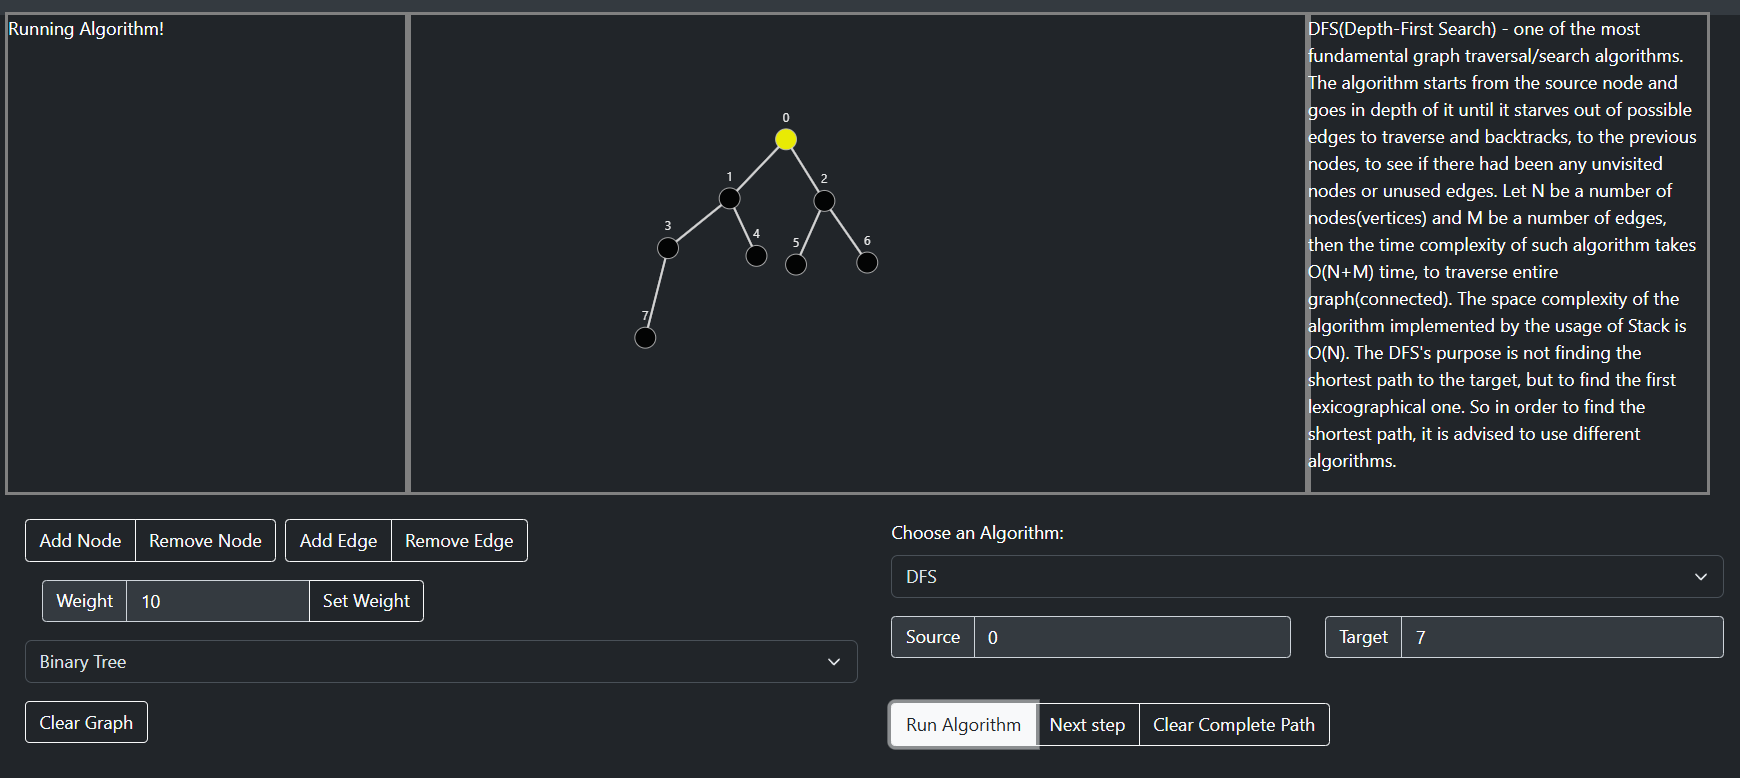
\includegraphics[width=\textwidth]{images/pressed_run_algo.png}
	\caption{After pressing run algorithm}
\end{figure}

After clicking on the button, algorithm will process one step. On figure 2.22, it is clear that the current processed node has changed, and the previously visited node is colored gray. One might find all of the nodes that have been visited during the time of execution being colored gray, as it is clearly the case. Gray nodes are already visited nodes.

\begin{figure}[H]
	\centering
	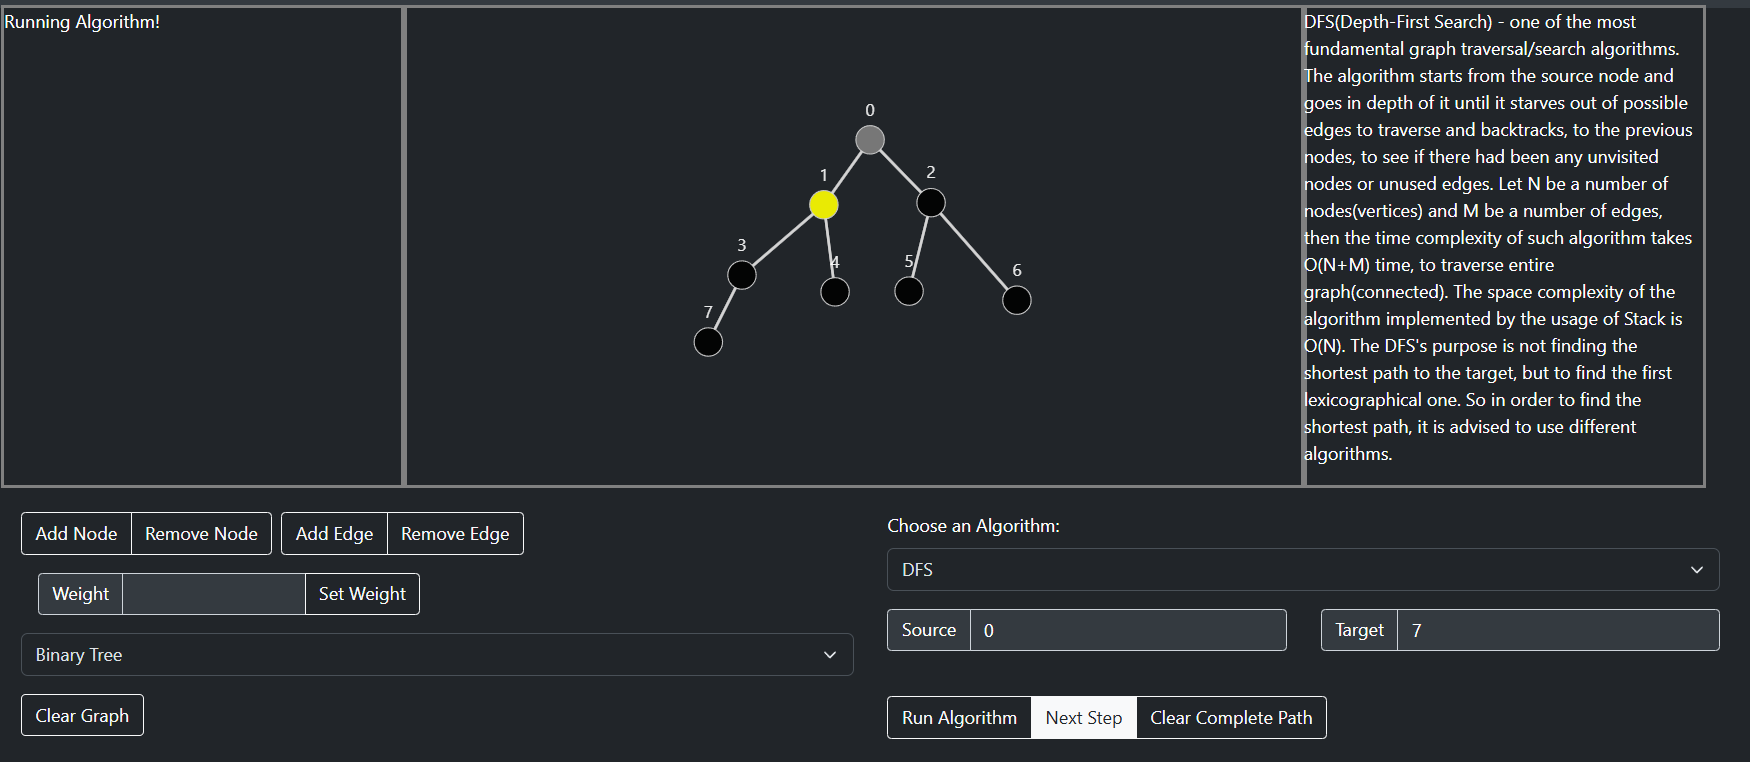
\includegraphics[width=\textwidth]{images/pressed_next_step.png}
	\caption{After pressing next step}
\end{figure}

Clicking on the "Next Step" button enough times concludes the final result of the chosen algorithm and results in the path found in the graph from source A to target B nodes. All of the nodes in the path are colored whether cyan or green, where cyan is used for the source and target nodes whereas green for all intermediate nodes of the path. Also, the path is printed out to the communication panel and its cost, in case we are dealing with the algorithm that finds an optimal path based on its weight accumulation.

\begin{figure}[H]
	\centering
	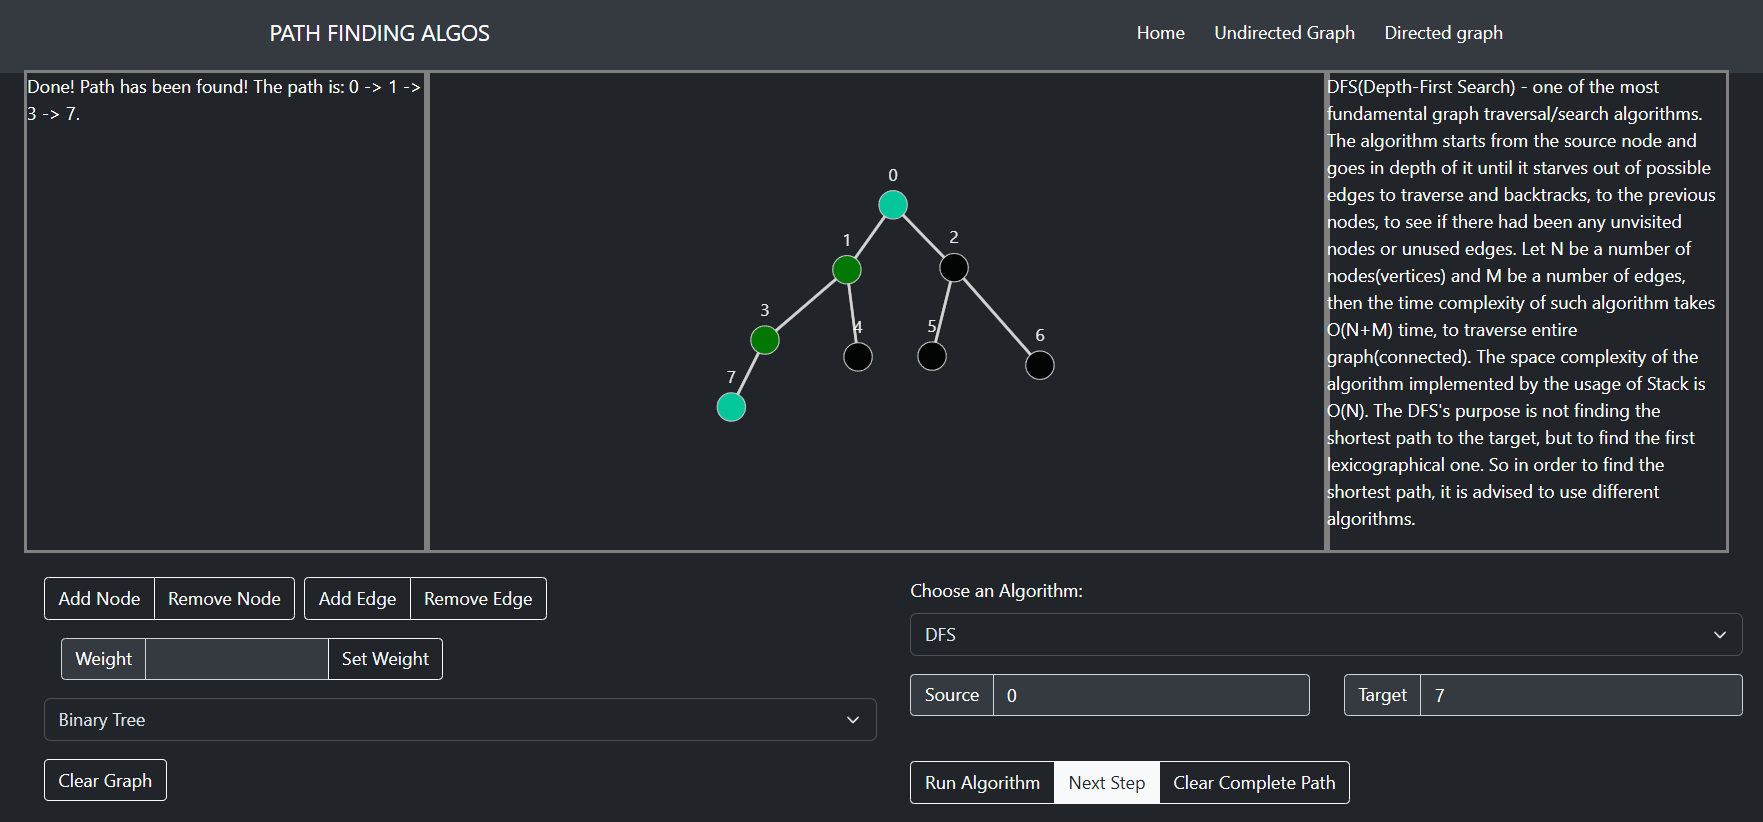
\includegraphics[width=\textwidth]{images/showing_complete_path.png}
	\caption{Completing algorithm}
\end{figure}

In order to get rid of the completed paths' coloring, learner can click on "Clear Complete Path" button. After that, all of the nodes regain their original black color.

\begin{figure}[H]
	\centering
	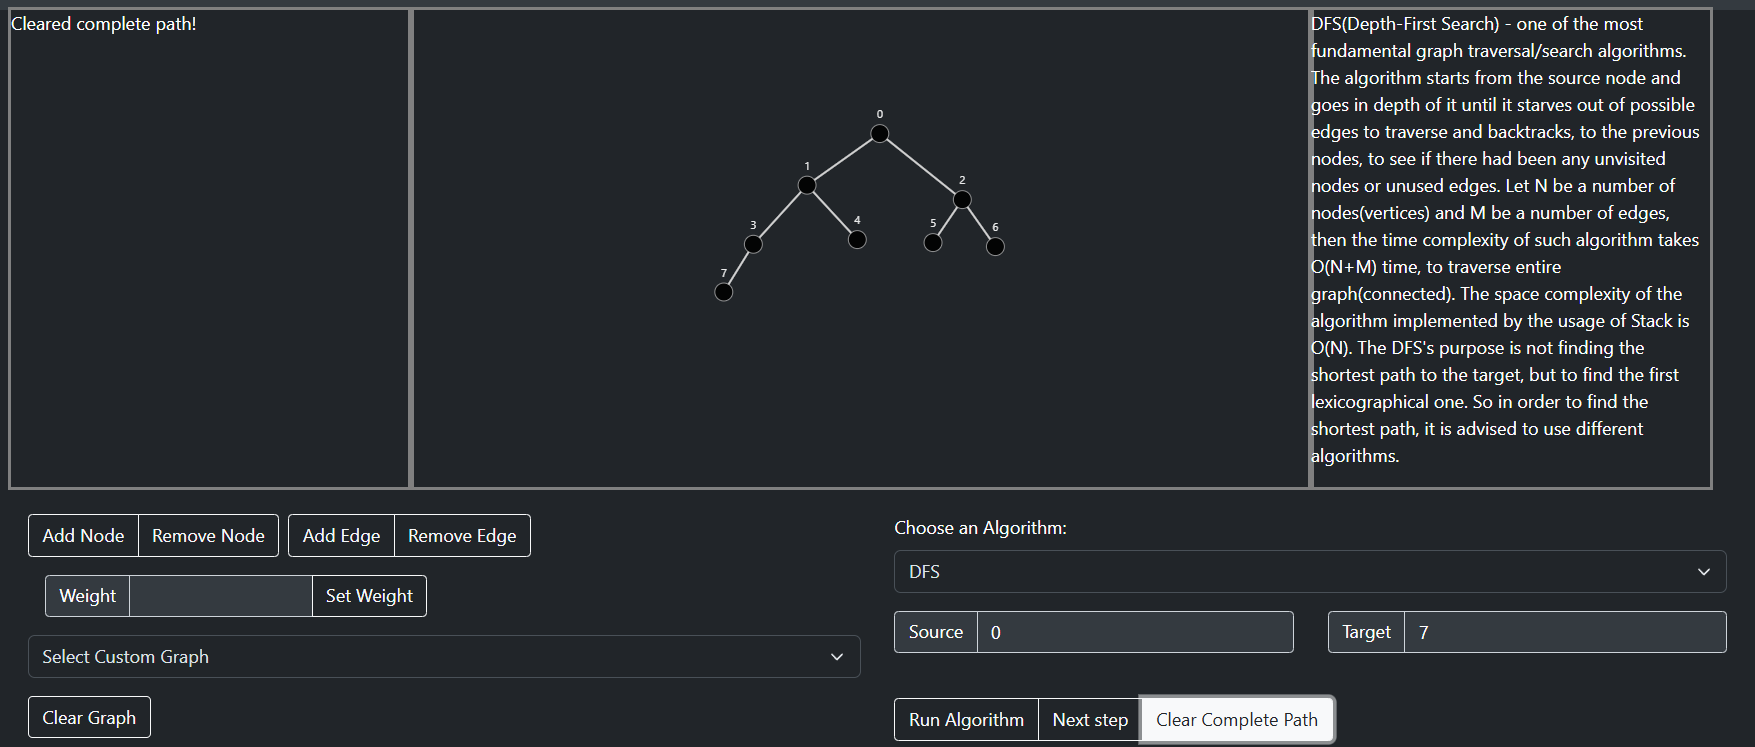
\includegraphics[width=\textwidth]{images/cleared_complete_path.png}
	\caption{Clearing the path}
\end{figure}

\subsection{Directed graph page}

As every example above has been showed on undirected graph, there is a directed graph page on figure 2.25, so that one sees what the different graph looks like.

\begin{figure}[H]
	\centering
	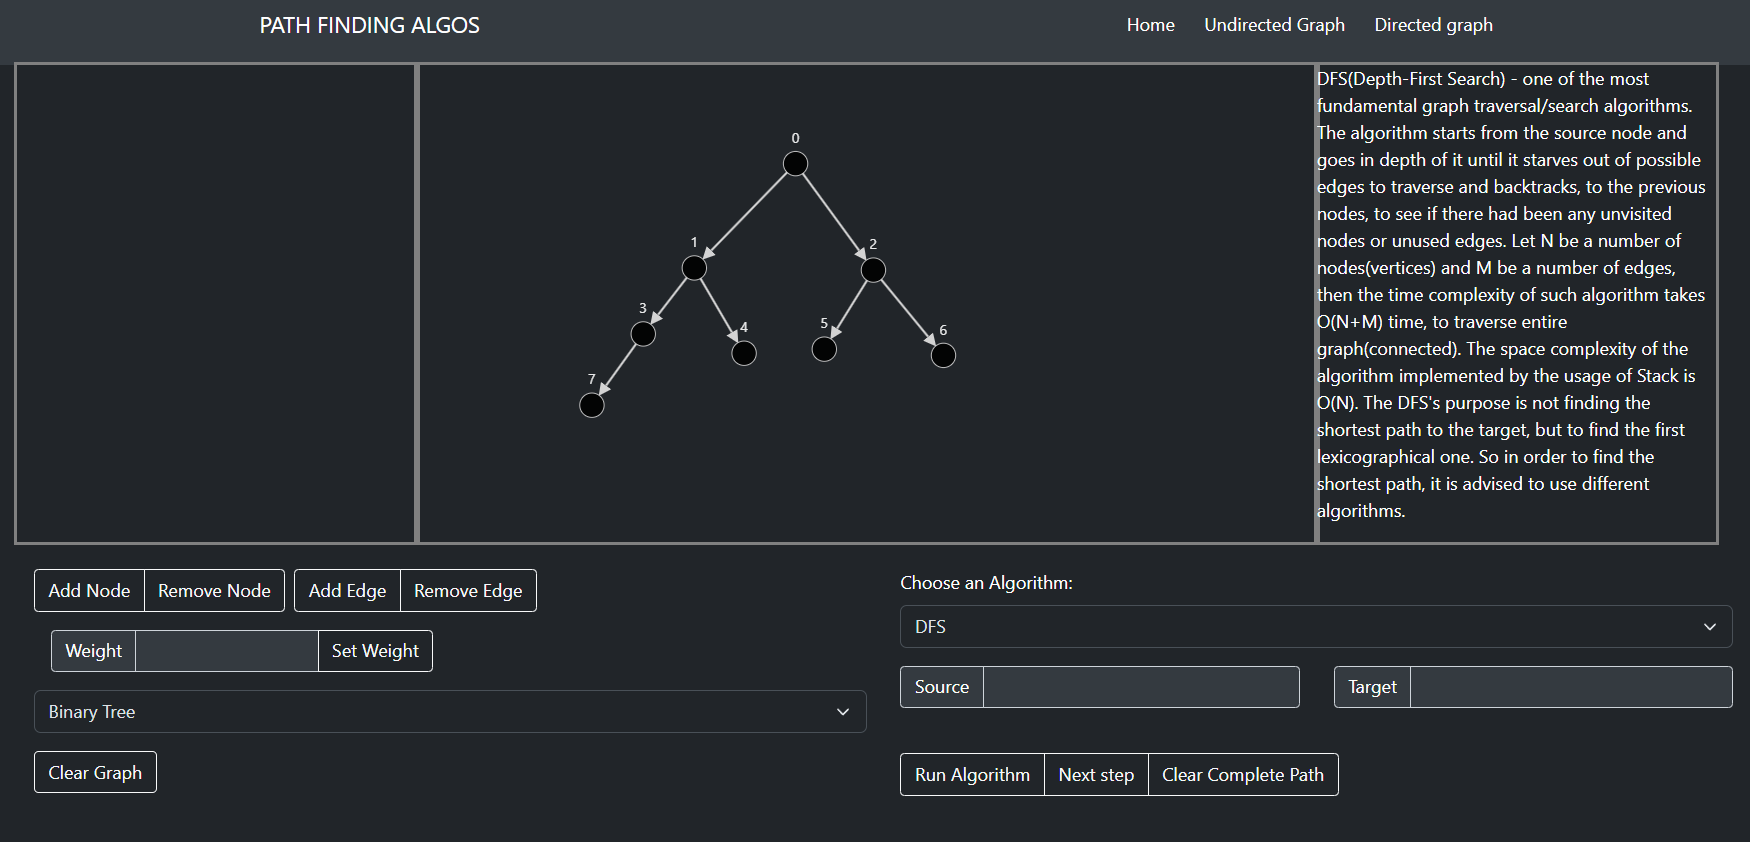
\includegraphics[width=\textwidth]{images/directed_graph.png}
	\caption{Directed graph}
\end{figure}


So far, it is all a learner needs to know about to proceed with the usage of tool. If one does not plan to change the behavior of the visualizer, then the next chapter is irrelevant to them. Various topics have been covered such as the graph, algorithm control and how one should make use of the communications inside the tool.
